\chapter{Setup}
When you launch fuelmanager for the first time, you need to select the type of database
you want to use and then add a vehicle.  There are two databases supported, sqlite and mysql.

\section{Configuration}
the configuration dialog looks like this:
  \begin{center}
    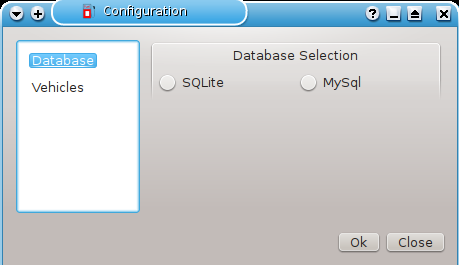
\includegraphics{snapshot11}
  \end{center}

\section{sqlite}
If you choose sqlite, you need to select the path of where the file will be located.
Then click apply to save the changes.
  \begin{center}
    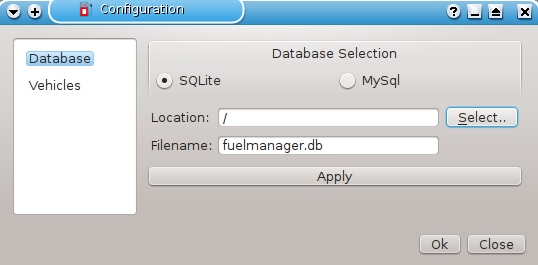
\includegraphics{snapshot2}
  \end{center}

\section{mysql}
If you choose mysql, you need to type in the hostname, port number, and the database name. 
Click apply to save the changes.  
  \begin{center}
    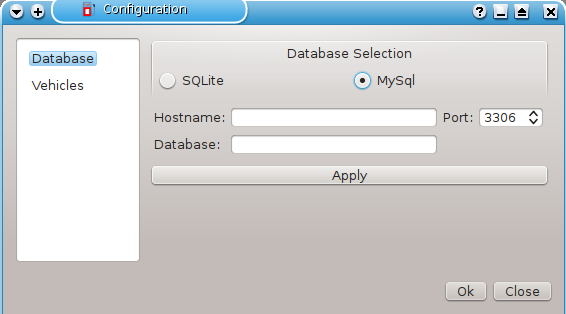
\includegraphics{snapshot3}
  \end{center}
  
\section{vehicles}
Click on the vehicles option on the left.
Type in the description in the description field and click apply to save the changes.
  \begin{center}
    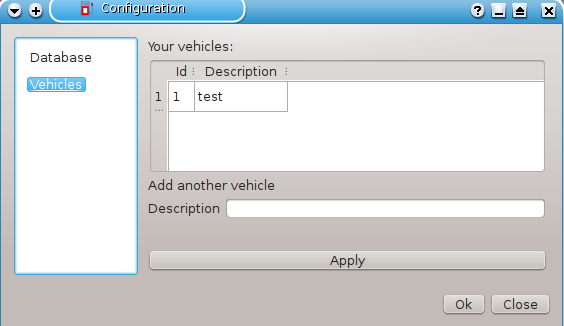
\includegraphics{snapshot4}
  \end{center}

\section{Setup Complete}
Setup is now complete, click ok to close the box.
